% !TEX root = main.tex
\section{Non-contextual Gaussian bandits: comparison to the Oracle TS}
\label{asec:noncontextual_gaussian_bandits}

\begin{figure}[!h]
	\centering
	\begin{subfigure}[b]{0.32\textwidth}
		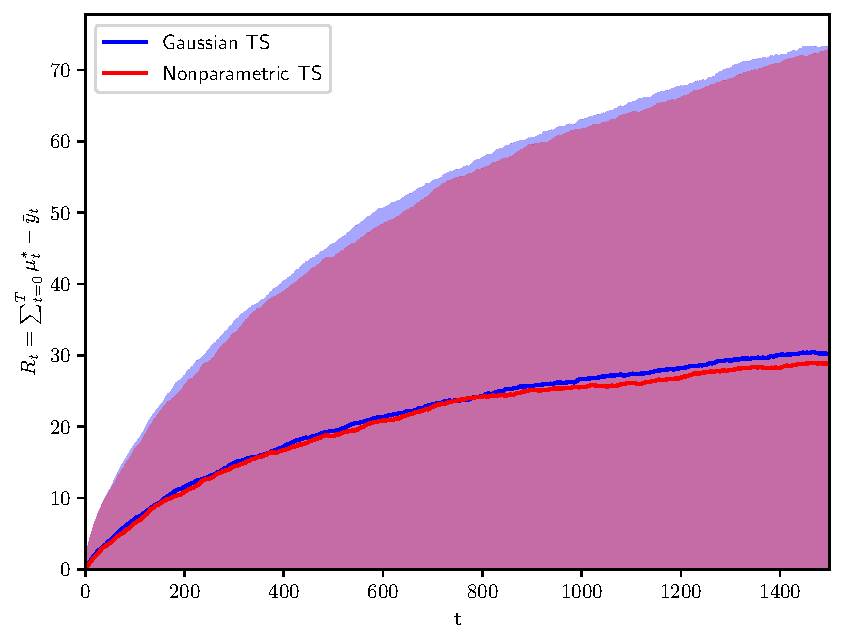
\includegraphics[width=\textwidth]{./figs/staticGaussian/cumregret_A2_-01_01_1_1}
		\vspace*{-5ex}
		\caption{$A=2$, $\theta_{1}=-0.1$, $\theta_{2}=0.1$.}
		\label{afig:static_gaussian_A2_01}
	\end{subfigure}
	\begin{subfigure}[b]{0.32\textwidth}
		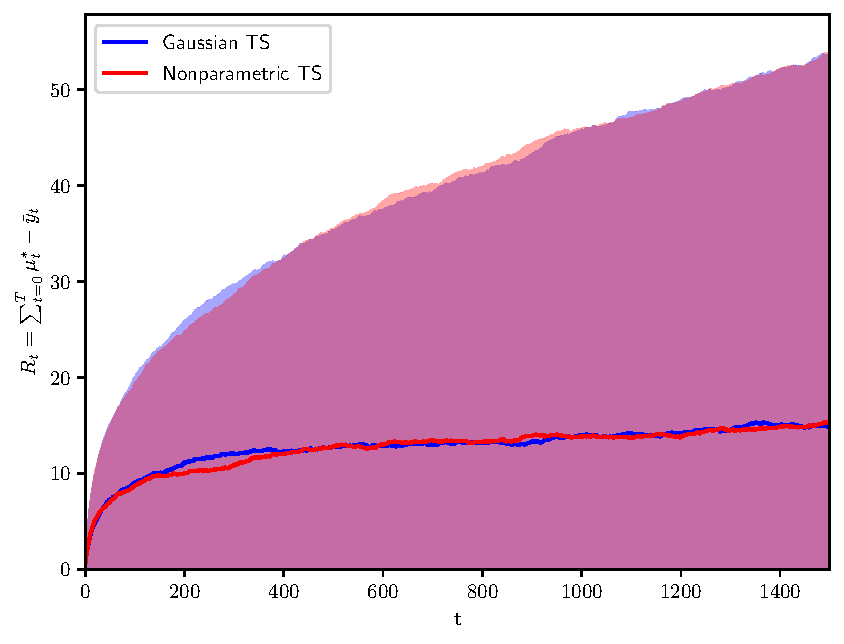
\includegraphics[width=\textwidth]{./figs/staticGaussian/cumregret_A2_-05_05_1_1}
		\vspace*{-5ex}
		\caption{$A=2$, $\theta_{1}=-0.5$, $\theta_{2}=0.5$.}
		\label{afig:static_gaussian_A2_05}
	\end{subfigure}
	\begin{subfigure}[b]{0.32\textwidth}
		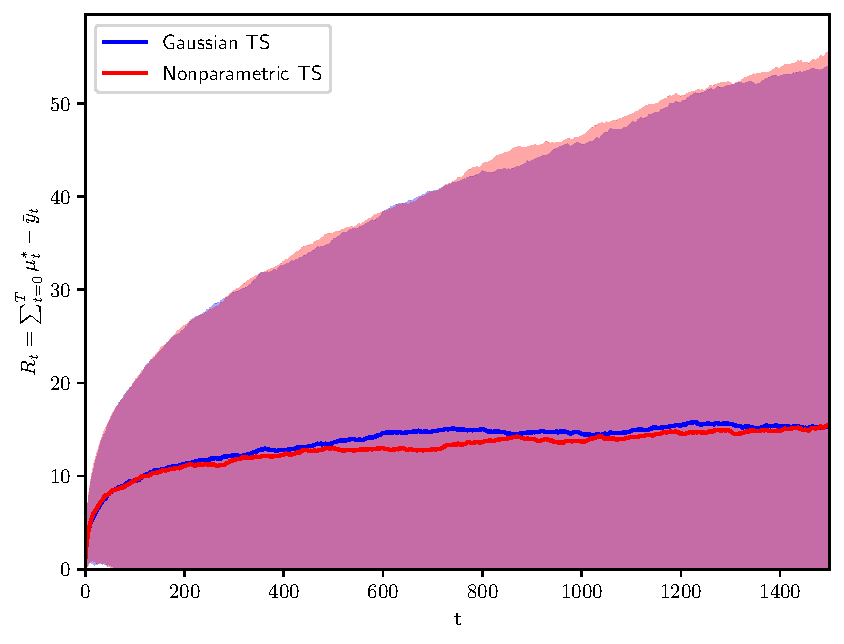
\includegraphics[width=\textwidth]{./figs/staticGaussian/cumregret_A2_-1_1_1_1}
		\vspace*{-5ex}
		\caption{$A=2$, $\theta_{1}=-1$, $\theta_{2}=1.0$.}
		\label{afig:static_gaussian_A2_1}
	\end{subfigure}
	\vspace*{-2ex}
	\caption{Mean regret (standard deviation shown as shaded region) for 1000 independent realizations of different two-armed Gaussian bandits, with $\sigma_a^2=1 \forall a$.}
	\label{afig:static_gaussian_A2}
\end{figure}

We show in Figure~\ref{afig:static_gaussian_A2} how our proposed nonparametric Thompson sampling method achieves regret comparable to that of the non-contextual Gaussian Thompson sampling as in~\cite{ip-Agrawal2012} for diverse parameterizations of such Gaussian bandits.

Recall that the non-contextual bandit scenario is seamlessly accommodated by our proposed \texttt{Nonparametric TS} algorithm by assuming a constant context, \ie $x_t=\mathds{1}$.